\documentclass{article}
\usepackage[utf8]{inputenc}
\usepackage[hungarian]{babel}
\usepackage{lmodern}
\usepackage[T1]{fontenc}
\usepackage{t1enc}
\usepackage{multicol}
\usepackage[a4paper, total={8in, 10in}]{geometry}
\usepackage{color}
\usepackage{amsfonts} 
\usepackage{mathtools} % \coloneqq
\usepackage{hyperref}

\usepackage[export]{adjustbox} % frame
\usepackage{listings}
\usepackage{color} %red, green, blue, yellow, cyan, magenta, black, white
\definecolor{mygreen}{RGB}{28,172,0} % color values Red, Green, Blue
\definecolor{mylilas}{RGB}{170,55,241}
\definecolor{lightgray}{RGB}{240,240,240}
\lstset{language=Matlab,%
	%basicstyle=\color{red},
	backgroundcolor = \color{lightgray},
	breaklines=true,%
	morekeywords={matlab2tikz},
	keywordstyle=\color{blue},%
	morekeywords=[2]{1}, keywordstyle=[2]{\color{black}},
	identifierstyle=\color{black},%
	stringstyle=\color{mylilas},
	commentstyle=\color{mygreen},%
	showstringspaces=false,%without this there will be a symbol in the places where there is a space
	numbers=left,%
	numberstyle={\tiny \color{black}},% size of the numbers
	numbersep=9pt, % this defines how far the numbers are from the text
	%emph=[2]{word1,word2}, emphstyle=[2]{style},	
}

\title{Audió fájl visszhangosítása hatékonyan}
\author{Vörös Asztrik}
\date{\today}

\begin{document}

\maketitle
\abstract{%
	Feladatom, hogy egy tetszőleges audió fájlt\footnote{pavarotti\_original.wav} visszhangossá tegyek, eleinte az egész fájl felhasználásával, majd szeletelve, ezzel real time működés feltételét biztosítva. Ehhez egy visszhangos teremben készített impulzusválaszra van szükség, hiszen ez leírja a szobát, mint rendszert, így bármilyen normál audió fájl átkonvertálható ebbe a rendszerbe. Gyakorlatban az impulzusválaszt egy, a szobában készített tapssal fogom közelíteni\footnote{impresp.wav}. \\
	\\
	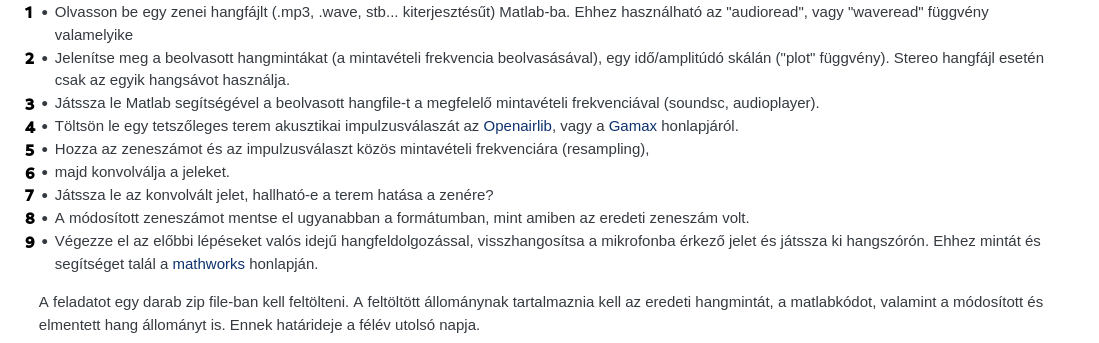
\includegraphics[width=\linewidth,frame]{image/feladat.png}
}

\section*{Matlab}
	A Matlab egy alapvetően mátrixokra épített programozási nyelv, mely rendelkezik azokkal a funkcionalitásokkal, melyek egy ilyen feladat elvégzéséhez praktikusak, ha rendelkezünk az adott csomagokkal. Szükségszerű, hogy a Matlab itt használt függvényeinek működésébe belemenjek felületesen, hogy érthetőek legyenek a megfontolások. Szintén célszerű a segédfüggvények taglalását is a lényegi résztől különvenni, így ezt is itt teszem meg. A dokumentum során taglalt függvények egyben szintén megtalálhatóak csatolmányként.
	\subsection*{fft, ifft, conv, nextpow2}\label{section:conv}
		Az \textit{fft(data, n)} függvény (Fast Fourier Transformation) diszkrét Fourier transzformációt (DFT) hajt végre, úgy hogy a végeredményként adott vektor mérete $n$ legyen\footnote{\href{https://www.mathworks.com/help/matlab/ref/fft.html\#d123e413321}{Matlab forum}} Az \textit{ifft(data)} ennek az inverzét hajta végre, azaz az inverz Fourier transzformációt.\\
		Mivel az fft algoritmus hatékonyabb futásidővel rendelkezik 2 hatvány méretű bemenetek esetén\footnote{\href{https://www.mathworks.com/help/matlab/ref/fft.html\#expand_panel_heading_f83-998360-n}{Matlab documentation: Input arguments: n}}, ezért az utóbbi paramétert arra fogjuk felhasználni, hogy a hossznál nagyobb $2^k\ (k \in \mathbb{Z})$ méretet adjunk meg (és célszerűen a legkisebb ilyet). Végül figyelnünk kell, hogy inverz Fourier transzformációkor a kimenet végéből levágjunk, hiszen a sebesség miatt extra üres adatokkal egészítettük ki a bementet. Mivel az időtartományban végzett konvolúció (\textit{conv(data$_1$, data$_2$)}) eredményének hossza $|$data$_1| + |$data$_2| - 1$ (mely ekvivalens a frekvenciatartomány elvégzett konvolúcióval visszaalakítás után), így az eredménynek a végéből a kiegészített mértéket kell levágnunk.\\
		Másik kiemelendő dolog, hogy DFT esetén a frekvenciatartománybeli szorzattal nem kaphatjuk meg (visszalakítás után) az időbeli konvolváltat a ciklikus tulajdonsága miatt. Azonban ha adott data$_1$ hosszát kiegészítjük $|$data$_2| - 1$-gyel akkor már nem tud átfedés történni (megszűnik a ciklikus tulajdonság), így ekkor ekvivalens lesz az időbeli konvolúcióval\footnote{\href{https://www.youtube.com/watch?v=eOvMUtMoQG8}{Levezetés}}\footnote{\href{https://www.mathworks.com/help/signal/ug/linear-and-circular-convolution.html}{Matlab help}}. \\
		Az előző kettő megállapítás után tudhatjuk, hogy a minimális hossz $|$data$_1| + |$data$_2| + 1|$, amihez keressük az első nála nagyobb egész kettő hatványt. Ez utóbbinak a kitevőjét a \textit{nextpow2} adja meg számunkra. Tehát a matlab beli kódunkban a következő fog szerepelni:
		\begin{lstlisting}
			nfft = 2^nextpow2(length(data1) + length(data2) - 1);
		\end{lstlisting}
	\subsection*{energy}
		A Parseval tételnek megfelelő energiáját számolja ki egy adatra.
		\lstinputlisting{code/energy.m}
	\subsection*{rescaleByEnergy}
		Energiamegtartó skálázást tesz lehetővé. Mivel az energiaszámításnál az adatok négyzeteit adjuk össze, így a kettő energiaaránynak a négyzetével skáláz. \\
		Erre azért van szükség, mivel konvolúció során a bemenetet egy másik függvény értékeivel szorozzuk, így ki fogunk esni az \textit{audiowrite} által wav fájlba írható vektor értékkészletéből ($[-1, 1]$)\footnote{\href{https://www.mathworks.com/help/matlab/ref/audiowrite.html\#expand_panel_heading_btiacgz-1-y}{Matlab documentation: Input arguments: y: Data Type of y: double}}.
		\lstinputlisting{code/rescaleByEnergy.m}
	\subsection*{rescaleChunk}
		A szelet méretének négyzetével osztja vissza az adatot. \textit{rescaleByEnergy} függvényt nem tudtam felhasználni real time működés esetén, így ott ezt a visszanormalizálást használom.\footnote{\href{https://numpy.org/doc/stable/reference/routines.fft.html\#normalization}{NumPy documentation: Normalization}} \\
		\textit{rescaleByEnergy}-nél említett okok miatt van rá szükség\footnote{\href{https://www.mathworks.com/help/audio/ref/audiodevicewriter-system-object.html\#expand_panel_heading_mw_de214585-205f-44e4-b3aa-88b50a0ae85a}{Matlab documentation: Input arguments: audioToDevice}}.
		\lstinputlisting{code/rescaleChunk.m}
	\subsection*{getAudioMono}
		Akár nem monó hanganyag betöltését teszi lehetővé.
		\lstinputlisting{code/getAudioMono.m}
	\subsection*{playAudio}
		Hanganyag lejátszását teszi lehetővé. Blokkoló utasítás, így megakadályozza, hogy a program végetérjen és a hanganyag félbeszakadjon.
		\lstinputlisting{code/playAudio.m}
	\subsection*{paddingZero}
		A vektort kiegészíti annyi nullával, hogy a megadott hosszt elérje a vektor hossza. Ha a megadott hossz kisebb a vektor hosszánál, akkor értesít erről a kimeneten.
		\lstinputlisting{code/paddingZero.m}
	\subsection*{paddingZeroMultiple}
		A vektort kiegészíti annyi nullával, hogy a hossza osztható legyen a megadott számmal.
		\lstinputlisting{code/paddingZeroMultiple.m}

\section*{1-3. feladat}
	A feladat egy wav fájl, kiplotolása és lejátszása volt. \\
	Beolvasáshoz a már korábban taglalt \textit{getAudioMono}-t használtam, mely megadja az adathoz tartozó mintavételi frekvenciát is (\textit{inpSampleRate}). \\
	A kirajzoláshoz ki kellett számolnom a teljes fájl hosszát és 2 adat között eltelő időt, a felhasznált adatok alapján. Mivel a frekvencia azt adja meg, hogy másodpercenként hány mintavételezés készült, így ha a teljes adat hosszát ezzel elosztjuk, akkor megkapjuk hány másodperces volt eredetileg. A 2 adat között eltelő időt például úgy is megkaphatjuk, hogy a hosszt elosztjuk az adatok számával, mivel azok között eltelő idő konstans. Ezután már csak a \textit{plot(x, y)} függvénynek meg kell adnia megfelelő formátumban az előbb kiszámoltakat. \\
	A hanganyag lejátszásához az \textit{audioplayer(data, sampleRate)}-et használtam, melyet nem aszinkron kell lejátszani (\textit{.playblocking()}), különben a program azonnal véget érne.
	\lstinputlisting{code/1-3.m}
	\begin{center}
		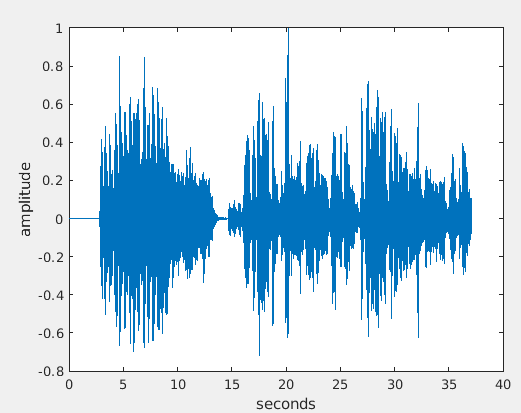
\includegraphics[width=\linewidth/2]{image/1-3.png}
	\end{center}
\section*{4-8. feladat: Teljes adatra végzett konvolúció}
	Miután a fájlokat beolvastam, a bemenetet és az impulzus választ közös frekvenciára hozzam a \textit{resample(data, p, q)} függvény segítségével, ahol az egyes adatokat $\frac{p}{q}$-val szorozza be a függvény. A konvolúciót el lehet végezni idő- és frekvenciatartományban, melyet a \textit{shouldConv}-val lehet állítani. Ezután újraskáláztam az értékeket, hogy a megfelelő értékkészletben legyenek. Ezeknek a működését a Matlab szekcióban lehet megtalálni. Végül \textit{audiowrite(src, data, sampleRate)} függvénnyel kiírtam az eredményt egy wav fájlba\footnote{pavarotti\_conv.wav}.
	\begin{lstlisting}
addEffect("pavarotti_original.wav", "echo.wav", "pavarotti_conv.wav", false);
	\end{lstlisting}
	\lstinputlisting{code/addEffect.m}
	Érdekes kísérlet volt az időtartományban és a frekvenciatartományban végzett konvolúció közötti időkülönbség. Az impulzus válasz 4 másodperc hosszú volt 48kHZ mintavételezés frekvenciával, az audió meg 3 perc 38 másodperc hosszú. Míg időtartományban számomra közelítőleg 6 perc volt, addig frekvenciatartományban közelítőleg 5 másodperc elvégezni a konvolúciót.

\section*{Overlap-add algoritmus}
	Overlap algoritmust arra tudjuk használni, hogy ne csak az egész fájl ismeretében végezhessük el a konvolúciót, hanem már annak szeletein is. Ezzel van lehetőségünk real time végezni az impulzus válasszal a konvolúciót. \\
	Az algoritmus lényege, hogy az egy szeletre elvégzett konvolúció eredményéből csak a szelet mérethez tartozó kezdő részt tekintjük a kimenetnek, a túllógást majd a további szeletek konvolúciós eredményéhez adjuk hozzá.
	\footnote{\href{https://www.mathworks.com/help/signal/ref/fftfilt.html\#mw_80e5adbd-8d4e-43f8-b26b-b417d8b80465}{Matlab help: Algorithms}}
	\footnote{\href{https://www.mathworks.com/help/dsp/ug/overlap-add-save.html}{Matlab help: Overlap add}}

\section*{9. feladat: Real time konvolúció}
	Ennek a feladatnak a megoldásához az overlap add algoritmust használtam. Sajnos a webes matlab nem képes a mikrofon kezelésére és az offline linuxos verzió nem támogatja megbízhatóan az audiokezelést. Emiatt először az előző feladatokban használt zenét szeleteltem fel, mintha realtime érkezne az adat és úgy teszteltem az algoritmus működését\footnote{pavarotti\_realtime\_simulated.wav}. Ezután az overlap algoritmust kiszerveztem egy másik függvénybe, hogy ezt a mikrofont használó megoldás is fel tudja használni. \\
	A függvények során gyakran egészítek ki a \textit{chunkSize} többbszörösére, mivel alapvetően chunk egységegben dolgozunk, ezzel megszűntetve lekezelendő speciális eseteket a kódolás során. A \textit{simulateRealTime} függvény ezeken kívűl nem tartalmaz újdonságot.
	\begin{lstlisting}
simulateRealTime("pavarotti_original.wav", "echo.wav", "pavarotti_realtime_simulated.wav", 2048);
	\end{lstlisting}
	\lstinputlisting{code/simulateRealTime.m}
	Az \textit{addEffectToChunk} függvény alapvetően az overlap add algoritmust hajtja végre. Kiemelendő, hogy első iterációban az \textit{overlap} hossza $0$ lenne, ezért ki kell egészítenünk minimum 1 \textit{chunkSize}-ra. Azonban ha pont 1 \textit{chunkSize} lenne, akkor a felhasznált overlap levágásakor szintén kezelendő szélső eset lenne, így érdemesebb annak a kétszeresére választani a méretet. Ezenkívül akalmazva van a már leírt \textit{rescaleChunk} és a szintén indokolt \textit{paddingZeroMultiple}. \\
	\lstinputlisting{code/addEffectToChunk.m}
	Végül találva egy reprodukálható működést megírtam a mikrofon alapú kódot is. Itt eleinte csak az impulzusválaszt olvastam be, majd annak frekvenciatartománybeli értékeit is kiszámoltam, hogy ne kelljen minden bejövő szeletnél újraszámolni. Ezután a beépített Matlab függvényekkel lekértem a mikrofont és a hangszórót leíró eszközöket. Végül a végtelenségig kérek a mikrofontól szeletet, amit átdolgozok az \textit{addEffectToChunk} függvénnyel, majd a hangszórón lejátszom az eredményt.
	\begin{lstlisting}
addEffectToMic("echo.wav", 2048, 44100);
	\end{lstlisting}
	\lstinputlisting{code/addEffectToMic.m}
	Tesztelésem során arra jutottam, hogy adott szeletméret esetén a következők tapasztalhatók az én konfigurációmon: 512 esetén a hang rossz minőségű, 1024 esetén késés figyelhető meg, 2048 egy jó választásnak tűnik, 4096-tól újra elkezd nőni a késés.

% egyben az egész
% calling codes

\end{document}
